\chapter{Modelli utilizzati}
%troppo poco come introduzione? o inutile?
Come abbiamo detto ci sono 3 tipi di modelli, il modello memoria, il modello router, e N sottomodelli autoencoder.

\subsection{Modello Memoria}
\begin{tikzpicture}[
	node distance=2cm,
	box/.style={
		draw,
		thick,
		rectangle,
		minimum width=1.5cm,
		minimum height=4.5cm,
		align=center
	},
	arrow/.style={-Latex, thick}
	]
	
	% Nodi
	\node[align=center] (input) {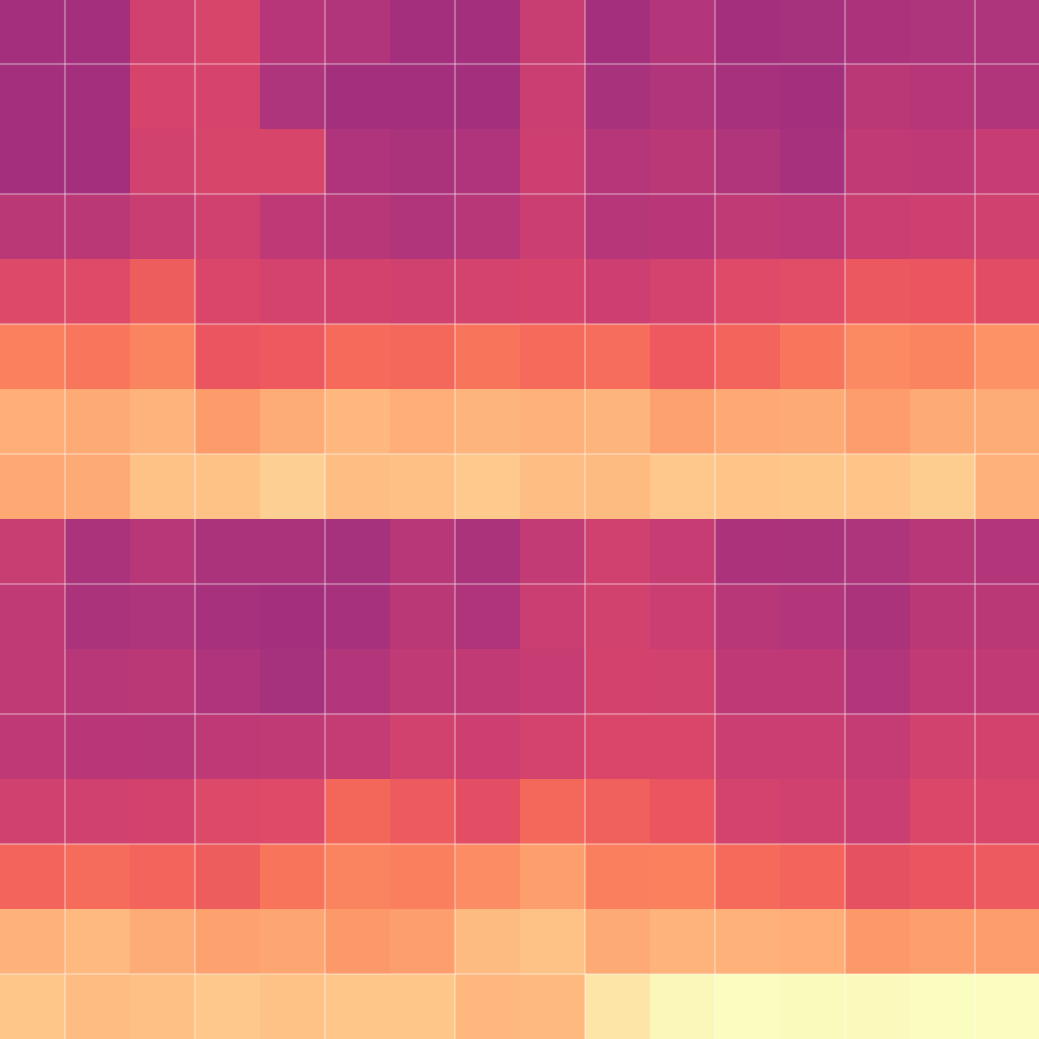
\includegraphics[height=2.5cm]{assets/images/spectrogram3.png}\\[0.2cm] Input};
	\node[box, right=of input] (lstm1) {\rotatebox{90}{LSTM Layer 1}};
	\node[box, right=of lstm1] (lstm2) {\rotatebox{90}{LSTM Layer 2}};
	\node[box, right=of lstm2] (output) {\rotatebox{90}{Output ($h_t$)}};
	
	% Connessioni lineari
	\draw[arrow] (input) -- (lstm1);
	\draw[arrow] (lstm1) -- (lstm2);
	\draw[arrow] (lstm2) -- (output);
	
	% Connessioni ricorrenti
	\path[arrow] (lstm1.north east) edge[out=70, in=110, looseness=3] node[above, font=\scriptsize] {Stato} (lstm1.north west);
	\path[arrow] (lstm2.north east) edge[out=70, in=110, looseness=3] node[above, font=\scriptsize] {Stato} (lstm2.north west);
	
\end{tikzpicture}

                       
	 \textbf{LSTM Memory Backbone} utilizza dei layer a Long Short Term Memory (LSTM) \cite{hochreiter1997lstm}, che permettono agli altri sottomodelli dicordare dati passati. Riceve in input i singoli segmenti dello spettrogramma e fornisce in output una rappresentazione latente dei dati. % ora che ci penso dovrei mettere controlli in caso di EGVG
	 Il modello memoria é condiviso con tutti i modelli che lo usano, quindi gli altri modelli devono essere allenati dopo il modello memoria.

\subsubsection{Modello router}                                                                                                                                                                                  
Il Router classifica i dati per selezionare l'autoencoder idoneo.                                                                                                                                
Le architetture usate sono:
\begin{enumerate}                                                                                                                                                                                                                    
	\item \textbf{Fully connected}:                                                                                                                                                                 
Rete neurale densa (Multilayer Perceptron, MLP) %altro da dire?              

	\item \textbf{STFT MCNN}:                                                                                                                                                           
Multi-branch Convolutional Neural Network. Applica reti convoluzionali parallele per estrarre caratteristiche dei dati diverse, usando kernel di dimensioni diverse \cite{zhang2016mcnn}.                                                                                                                                                        
         
	
	\item \textbf{1D CNN}
	Rete convoluzionale (multilivello) ad un kernel per livello che scansiona lo spettrogramma, ha un MLP finale per la classificazione.                                                                 
\cite{kiranyaz20151dcnn}
\end{enumerate}                                                                                                                                                                                                                      
\subsubsection{Modelli autoencoder}                       
%troppo prolisso/confuso?
Provano a ricostruire il segnale di input, la ragione per cui sono utili nel contesto dell'anomaly detection è che riescono a ricostruire il segnale di input solo se sono stati allenati con dati i a quelli che dovranno poi ricostruire, questo fa si che se incontrano dati mai visti non riusciranno a ricostruire in maniera affidabile l'input, e quindi possiamo assumere che quell'input è diverso in struttura dai dati in cui è stato allenato.

%TODO aggiungere disegno esplicativo di un AE?
\begin{enumerate}                                                                                                                                                     
	\item  \textbf{Autoencoder denso}:
	Usa semplici layer densi, essendo di fatto un MLP con dei layer di bottleneck, che formano lo spazio latente, tra l'encoder e il decoder
	
	\item \textbf{Variational
		autoencoder}:
		% si capisce? troppo corto
		Un VAE è, a livello strutturale, un autoencoder denso, tuttavia nella fase di training, si forza lo spazio latente ad essere formato da una distribuzione normale   $\mathcal{N}(0, 1)$ di $\mathcal{N}$ dimensioni. Questo permette allo spazio latente di non avere buchi, ovvero zone che producono in fase di decode dati incoerenti \cite{kingma2013auto}.
		
		
	\item \textbf{Convolutional Autoencoder 1D}:
	Usa layer convoluzionali in fase di encode, e layer deconvoluzionali in fase di decode. Utilizza come input lo spettrogramma interpretato come una serie multivariata, dove i singoli bin di frequenza fungono da canali di input. Il filtro convoluzionale scorre esclusivamente lungo l'asse orizzontale.
			
			
	\item \textbf{Convolutional Autoencoder 2D}:

	Usa layer convoluzionali in fase di encode, e layer deconvoluzionali in fase di decode. Utilizza come input lo spettrogramma interpretato come una vera e propria immagine spaziale a singolo canale.
	\item \textbf{Convolutional LSTM Autoencoder}:                                                                                                                                                   
Combina layer convoluzionali (per le feature spaziali) e celle LSTM (per le feature temporali) per catturare anomalie spazio-temporali  \cite{shi2015convlstm}.                         
\end{enumerate}                                                                                                                                                                                                                      
